% 2007 年新课标卷文科第 17 题：河对岸塔高 AB 的测量示意图。
%   C、D 在同一水平面内的近岸，B 为塔底（对岸），AB 为塔高；
%   A—C、A—D 为视线（虚线），C—D 为近岸基线，B—C、B—D 为水平距离。
% 来源 PDF：gaokaomath-src/普通高考/2007/2007新课标文(海南,宁夏).pdf
% SHA-256：c8ee1632ac3a7a28aab1150f047a2e1c74398ca2944701e9165237897ae724e2
% 原页：2007新课标文(海南,宁夏).pdf 第 1 页（A3 三栏）第 3 栏，书页码 393。
% 重绘依据：按原页塔、河岸、测点与视线的相对位置重绘，尺寸关系不按比例。
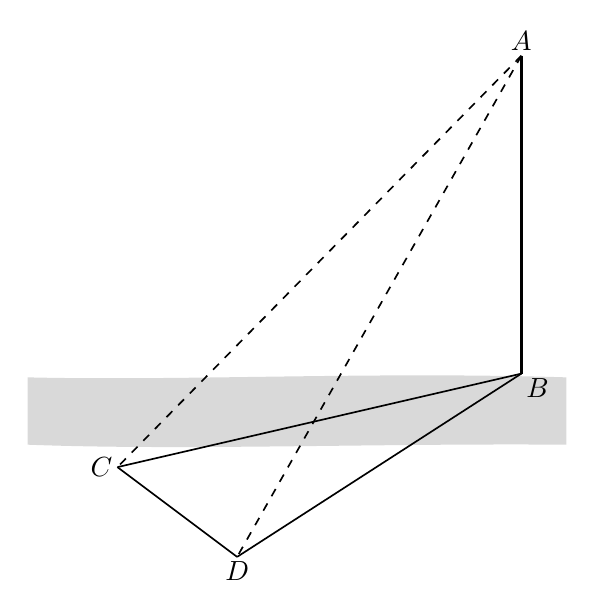
\begin{tikzpicture}[scale=0.95, semithick,
  every node/.style={inner sep=1.5pt}]

  \coordinate (B) at (4.0,0.95);
  \coordinate (A) at (4.0,5.2);
  \coordinate (C) at (-1.4,-0.3);
  \coordinate (D) at (0.2,-1.5);

  % 河面（近岸与对岸之间的灰色带）
  \fill[gray!30]
    (-2.6,0.0) .. controls (-0.5,-0.08) and (2.0,0.02) .. (4.6,0.0)
    -- (4.6,0.9) .. controls (2.0,0.98) and (-0.5,0.85) .. (-2.6,0.9) -- cycle;

  % 塔
  \draw[line width=1.1pt] (A) -- (B);
  \node[above] at (A) {$A$};
  \node[below right] at (B) {$B$};

  % 水平基线与视线
  \draw (C) -- (D);
  \draw (B) -- (C);
  \draw (B) -- (D);
  \draw[dashed] (A) -- (C);
  \draw[dashed] (A) -- (D);

  \node[left] at (C) {$C$};
  \node[below] at (D) {$D$};
\end{tikzpicture}
